\phantomsection
\addcontentsline{toc}{section}{Introduction}
\section*{Introduction}

Quantum Computing is a methodology of computation that harnesses quantum mechanics. The concept of simulating quantum-mechanical systems using a computational device has been around for over 40 years, \cite{feynman_1982} however, it is only recently that the technology has matured enough to show its potentially disruptive qualities. Their inherent parallel nature and exponential scaling with size means that it can solve problems outside the problem space of classical computers. The four main areas it has an advantage  are: combinatorial optimisation, linear algebra, differential equations and factorisation. Differential equations are particularly useful in nearly all aspects of computer modelling. Specifically, I will be looking at their usage in the modelling of biological molecules.


\phantomsection
\addcontentsline{toc}{subsection}{Fundamentals}
\subsection*{Fundamentals}

\phantomsection
\addcontentsline{toc}{subsubsection}{Classical Computing}
\subsubsection*{Classical Computing}

Classical Computing, or Binary Computing, is what underpins all of our current computer systems. Information in these systems are represented in units called bits \cite{bit_definition}. Physically, these units are represented by transistors, which are small electrical switches, that can store a charge. When the transistor is ``full'' of charge, that represents that bit being ``on'', or in the Binary number system, 1. When the transistor is ``empty'', that represents the bit being off, or a 0. These switches can be combined with other components to create logic gates \cite{logic_gate_definition}, and then our modern computer systems are built from these basic gates.

\phantomsection
\addcontentsline{toc}{subsubsection}{Quantum Computing}
\subsubsection*{Quantum Computing}
Similar to Classical Systems, Quantum Computers are based on ``quantum bits'', or Qubits. However, unlike classical bits, qubits are two-dimensional vectors. Graphically, this can be represented using a Bloch sphere. See \autoref{fig:bloch_sphere}.

\begin{figure}[H]
	\centering
	\[ 0 \rightarrow | 0 \rangle = \begin{bmatrix} 1 \\ 0 \end{bmatrix} \]
	\vspace{-0.2cm}
	\[ 1 \rightarrow | 1 \rangle = \begin{bmatrix} 0 \\ 1 \end{bmatrix} \]
	\caption*{Mapping of Classical Bits to Dirac notation \cite{dirac_notation} and column vectors}
\end{figure}

\begin{figure}[H]
	\centering
	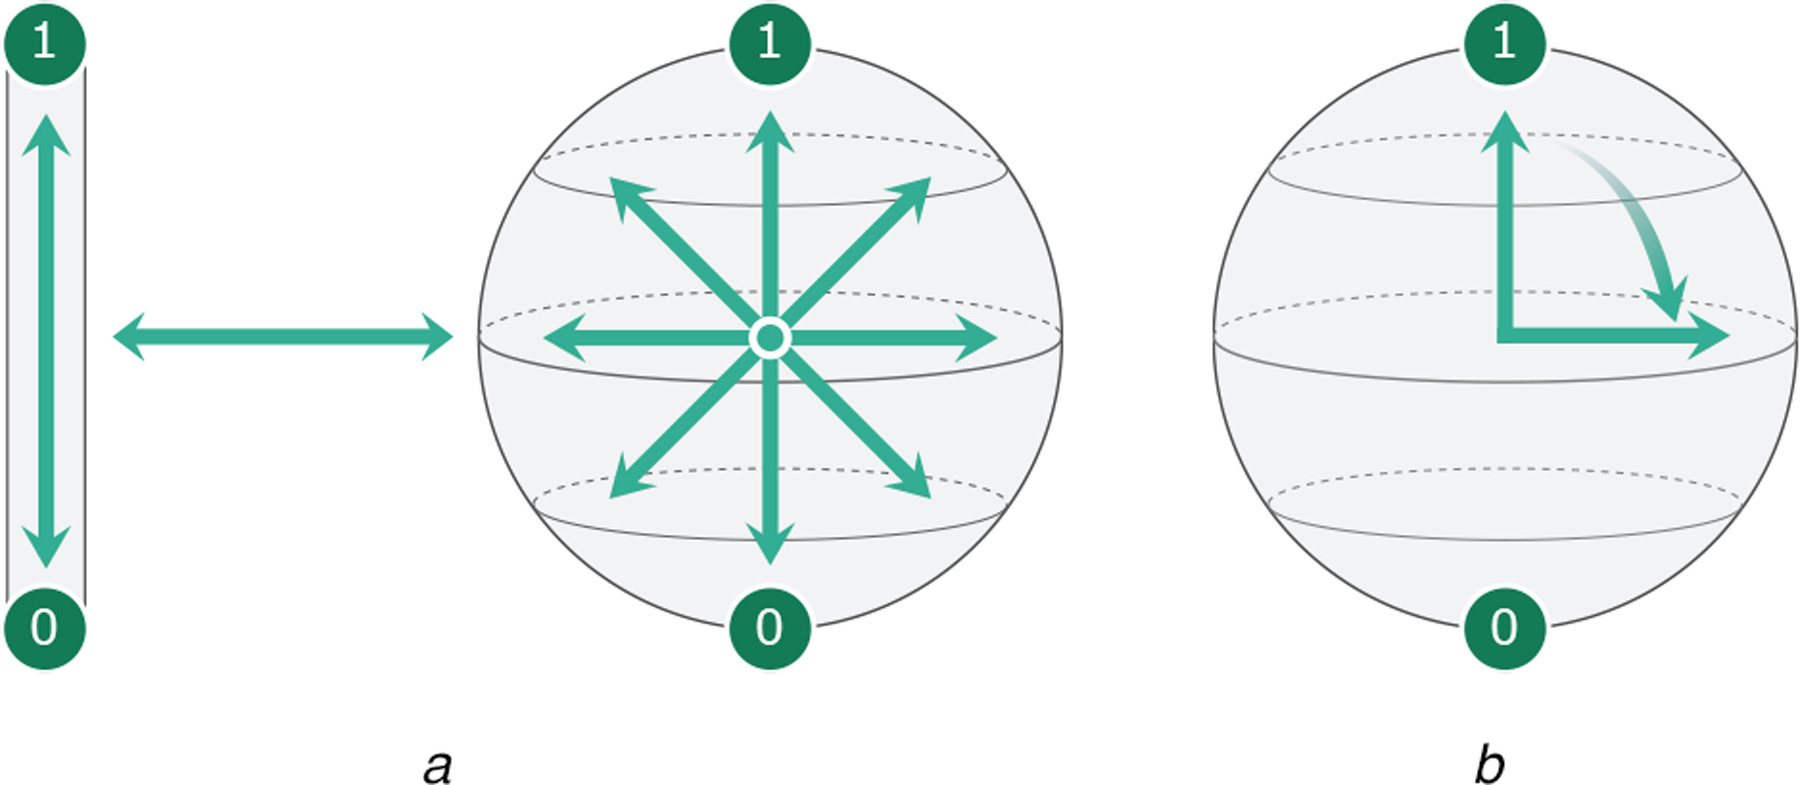
\includegraphics[width=0.65\textwidth]{blochsphere.jpg}
	\caption{a. Graphical Representation of a Qubit b. Hadamard Gate \cite{present_landscape_q}}
	\label{fig:bloch_sphere}
\end{figure}

The qubits $|0\rangle$ and $|1\rangle $ are referred to as $\{|0\rangle, |1\rangle\}$, the computational basis. This is the two basis states composed by any of the two distinct quantum states that the selected implementation of qubit can physically be in. For example, if we were using the spin \cite{quantum_spin} of a proton, where spin-up is our $|0\rangle$ state, and spin-down is our $|1\rangle$ state, then the computational basis of this qubit would be $\{|\uparrow\rangle, |\downarrow\rangle\}$.

Where qubits diverge from their classical analog is that qubit states are not discrete, meaning that they are not 0 OR 1. Instead, they exist in a superposition \cite{superposition} of both $|0\rangle$ and $|1\rangle$ states. When the value of the qubit is measured, it ``collapses'' to either $|0\rangle$ or $|1\rangle$. Whilst it cannot be predicted which state the qubit will collapse, the probability of whether a qubit will collapse to a particular state can be determined.

Analogous to classical computing, quantum computers also have quantum gates, which transform the input qubit, and large sequences of these gates can be used to perform more complex operations. More specifically, a quantum gate specifies how the computation basis (for example, $\{|0\rangle, |1\rangle\}$) is transformed by the operation of a quantum gate. The most common quantum gates are the \texttt {NOT(X)}, Hadamard gate and \texttt {CNOT(CX)}. The \texttt {NOT} gate transforms $|0\rangle$ to $|1\rangle$, and vice versa. The Hadamard gate creates an equal superposition state, therefore meaning that the input qubit has an equal chance to collapse to $|0\rangle$ or $|1\rangle$. Graphically, we can represent this by a rotation of $\pi^c$ in the Bloch Sphere \cite{bloch_sphere} (\autoref{fig:bloch_sphere}).

\phantomsection
\addcontentsline{toc}{subsection}{Computational Biology}
\subsection*{Computational Biology}

Computational Biology is the use of mathematical modelling and simulations to understand biological molecules and interactions between those molecules, and aims to analyse and visualise the complex connections in biological processes.

One major usage of this is in protein `folding', which is the prediction of the structure of a protein from its ammino acid sequence. This was particularly useful when modelling the viral proteins of SARS-CoV-2, due to its rapid mutagenesis, and allowed for mutations of the virus to be tested against vaccines and treatments without having the specific variant in a lab \cite{biom12111665, modern_techniques_cov}.

This is just one example of what we can use computational biology for; there are potentially limitless applications, such as simulating new fertilizers and personalising medicines. If we can successfully simulate biological molecules interacting given a set of starting conditions, in a timeframe quicker than it would take to observe the actual system, then the cost and time taken to develop new pharmaceuticals could be dramatically decreased. Drug molecules could be designed to interface perfectly with the intended recipient's body to ensure maximum efficacy. It would remove the need to prototype tens if not hundreds of molecules, as any error in the mdlecule would only require the simulation being ran again, rather than having to wait for the physical system to interact again.

The potential benefits of having the capabilities to simulate any system with any number of variables are therefore very obvious. 

